\documentclass[minf,frontabs,twoside,singlespacing,parskip]{infthesis} 

\usepackage{url}
\usepackage{graphicx}

%\usepackage{biblatex}
%\usepackage[xetex]{graphicx}
%
%\usepackage{fontspec,xunicode}
%
%\defaultfontfeatures{Mapping=tex-text,Scale=MatchLowercase}
%\setmainfont[Scale=.95]{Georgia}
%\setmonofont{Georgia}


\usepackage{amsmath}
\newcommand{\BigO}[1]{\ensuremath{\operatorname{O}\bigl(#1\bigr)}}


\usepackage{listings}
\usepackage{color}

\definecolor{dkgreen}{rgb}{0,0.6,0}
\definecolor{gray}{rgb}{0.5,0.5,0.5}
\definecolor{mauve}{rgb}{0.58,0,0.82}

\lstset{frame=tb,
  language=Python,
  aboveskip=3mm,
  belowskip=3mm,
  showstringspaces=false,
  columns=flexible,
  basicstyle={\small\ttfamily},
  numbers=left,
  numberstyle=\tiny\color{gray},
  keywordstyle=\color{blue},
  commentstyle=\color{dkgreen},
  stringstyle=\color{mauve},
  breaklines=true,
  breakatwhitespace=true
  tabsize=4
}


\begin{document}
\title{Modelling search volumes as a dynamic system responding to external events}

\author{Stefan Sabev}

\course{Master of Informatics}
\project{{\bf MInf Project (Part 1) Report}}

\date{\today}

\abstract{
It is well known that some events might spark people's interest to fly to different destinations. In particular news events or sports events can quite easily make people search for a specific destination - for example the Champions League Quarter final draw increased the number of flight searches from Glasgow to Spain 6 times.\\
For this project we have collected vast amounts of Twitter data. With this dataset and the flight search dataset provided by Skyscanner it was possible to build a classifier that predicts flight search demand based on what's happening on Twitter. This is a noble approach to predicting flight search volumes utilising the vastness of Social data available. \\
The potential applications of this are generic prediction of flight search volumes, predicting new events for better marketing and also anomaly detection in traffic caused by events.
%The main goal of this project is to collect Twitter data initially and possibly several other news sources and extract the available event data. Afterwards we'd want to split it into two groups - those who spark people's interest and those don't.
%This can later be used to detect when people want to go somewhere based on the news channels around the world.
}

\maketitle

\section*{Acknowledgements}

I would like to thank Charles Sutton for his support while supervising this project.\\
\\
Another thank you goes to Ewan Nicolson for helping with the project and giving access to data storage and the Skyscanner dataset used in this project.

\tableofcontents

\pagenumbering{arabic}



\chapter{Background}


With millions and some with billions of users, Social Networks are becoming an increasingly more important in our lives. A big proportion of people use it as their primary way of communicating with the outside world - people will "tweet" about anything, post to Facebook, check in on FourSquare, instagram their food and so on. We have become perfectly fine with externalising our lives and posting every minute detail about our lives online and thusly making it available to everyone else. 
Of course, there are always exceptions. After all 82\% of the population are not on Facebook, but those 1.23 billion monthly active users are all using it. Not all of them are avid users and post all of their pictures to it, but a big proportion is. With this amount of data on one's behaviour, life patterns and activities, companies can build a very good understanding of every individual. 


As with any other network - be it TV, radio, newspaper - there are always going to be some who are trying their best to commercialise it and benefit from it in some way. Since people are willing to share so much information about themselves online, there are terabytes of data being generated every day on what people did, what things they tweeted about, their latest pictures, etc. As we are entering the "Big Data" age where every company is trying to turn its data into a product or simply establish itself as the leading data supplier for a particular market. Due to the vastness and volumes of the data that these social networks generate they have sprung an entirely new eco-system of its own - companies are now plugging into Twitter, Facebook and all the other networks to figure out everything they can about you. Everyone is now talking about "sentiment analysis" in social media for brands, targeting particular demographics with ads on Facebook, promoting tweets and segmenting the customers into different groups and selling their data to marketers.


A particularly interesting one of that new generation of networks is Twitter. With a base of 200+ million active users it has slowly but surely become one of the most prominent sources of information and news on the web. It's previously beaten traditional news sources on numerous occasions by a few minutes when delivering the latest developments such the Los Angeles earthquake in 2008. \cite{TwitterNewsWire} They have their data streams opened up to developers and researchers as well, which is a fantastic opportunity to mine this data set for valuable information. There are plenty of articles on the internet on what people have done with it - demographics research, predicting flu outbreaks, etc. \cite{TwitterResearch} Miles Osborne here at the University of Edinburgh has done quite a lot of research using the Twitter data streams  \cite{Miles} and perhaps the biggest use is in Sasa Petrovic's PhD thesis. \cite{Petrovic2012}


In order to get more familiar with the trending events I have done read a few papers on Topic Detection and Tracking and First News Detection in order to see if I could use and extend it for my case. I'd like to mention Sasa Petrovic's PhD thesis as an excellent paper on the matter. \cite{Petrovic2012} However after careful investigation into the complexity of TDT I decided that this will be implemented in the 2nd part of the project, since I needed to familiarise myself with the dataset, try to see if there is more intelligent filters on the data stream and see how exactly they can be correlated to my 2nd dataset.


The only thing that has been researched in the online travel sector is what is the optimal time to book an airline flight taking into account all the different factors. \cite{Hamletkdd03} \cite{ijcai} 
Both of the referenced papers are using small sets of data which aim to predict what is the optimal time to book. What is written there is the other part of the puzzle - when should you book, but in this particular project we are more interested in when ARE people looking for flights.

\section{Brief outline}


Due to the lack of any research in this particular area setting the objectives for this project was very difficult. Planning on how to approach and tackle was in itself a challenge. There is no current proposed method of doing this, so there was no gold standard against which I could benchmark. That made it particularly hard to see whether the classifier is right or wrong and what should I strive to beat.


In the Introduction chapter \ref{chap:intro} on page \pageref{chap:intro} the problem is set out in detail as are the main reasons for this undertaking all together. There is also a synopsis of the results and an overview of what was done and achieved during this 1st phase. 


The Methodology can be found in chapter \ref{chap:method} on page \pageref{chap:method} split by all the main subtasks that had to be carried out. The subtasks are described in detail and each one of the sections includes an overview of what was done, how it was done and what difficulties were encountered and how I overcame them. 


Chapter \ref{chap:model} on page \pageref{chap:model} explains what are the Machine Learning models used to carry out the work for this project. Since there is no model defined anywhere I had to use an in-house algorithm used by Skyscanner to predict the search volumes. It's then described in depth which model worked best and why. 


In chapter \ref{chap:future-work} on page \pageref{chap:future-work} I discuss all the future work that will be carried out for this project both for next year and if someone is to pick it up and start developing on top. In order to do that I have included links to the source code for this project and all the pre-aggregated data sets from Twitter in the repository.



\chapter{Introduction and synopsis}
\label{chap:intro}


\section{Introduction}


There aren't that many flight search companies that aggregate massive volumes of data. And even further ones that are making some or all of their data sets available for research. When you consider that and the fact that online travel is a niche area in itself, one might start to understand why a project of this kind would be quite hard if not impossible to do. However as most of those companies grow, they are trying to employ more sophisticated ways of predicting demand and as a result of that their capacity. With the rise of social media, the next logical step for some of them start to explore different ways of adding exogenous factors such as twitter data their predictions. 


This project is the first time that someone has actually tried to correlate these two distinct types of data sources together and use social media to measure the effect it has on online travel. We will try to show that using this dataset (\textasciitilde 480GB at the time of writing) we can employ text mining and try to build a classifier that can predict upward and downward shifts in dement on certain airline routes. That will allow more flexibility and give a better understanding of what actually drives demand, so it could be useful not just to Skyscanner, but to airlines and airports as well.


It will be impossible not to say anything about Skyscanner, since my 2nd dataset is from it.  \footnote{\textbf{Dislaimer}: I am an employee of the company and have been working there since 2011} It's an Edinburgh-based company with offices around the whole world. It has been in a phase of rapid growth in the past couple of years doubling in size every year.
Skyscanner has always been a data-driven company. It's one of the few in this industry that are actually growing instead of stagnation. The growth of the data they generate and store follows a similar pattern, but the increase there is even bigger - the company is serving billions of searches every month. 


This particular project was spurred after a discussion that social media could be harnessed to produce aggregate numbers which will allow us to see whether there are going to be any expected spike to any destinations. Of course that will not be a "one size fits all" approach, since some places such as London, Paris and New York will see steady very high number of search volumes to them. The destinations that are thought to be better predicted by the classifier with Twitter are the ones that are not constant all year round - Ibiza, Alicante, Dubrovnik and many others. Those destinations have a particular seasonality with spikes around holidays and some events. 


The proposed way of taking this is to mine the vast quantities of Twitter data collected in a particular fashion (all ways described in chapter \ref{chap:method} on page \pageref{chap:method}) and take the numbers produces as the what we will call the "Twitter counts" for a particular city or overall. We will aim to beat the classifier for those more seasonal destinations that are not as well predicted by the in-house standard method. The approach described here could be used to develop a system that monitors the social streams and is can be used as a weight in the in-house predictors.


In the first part of the project I have taken a pragmatic approach and explored the most practical use - predicting search volumes for all the destinations mentioned on Twitter with the Twitter counts and a features which are automatically picked from the Twitter Stream. All the datasets are made available in the GitHub repository. \cite{code} Of course because of confidentiality I can't publish the dataset which has the Skyscanner searches, since that might break my employee code of conduct. Instead I have anonymised it by normalising as described in the methodology. 


When the project is extended to be a more real-time system with some TDT the potential applications of it are quickly increasing in numbers. In theory, one can monitor what is happening and what is trending and as soon as something relevant is seen - event in a different country/city or in general something happening in a country one can action in a multitude of ways:
\begin{itemize}
\item "X is happening, why not fly there to see it?"
\item Develop it further to monitor social media in order to predict spikes in traffic. Appearance on Italian TV caused half an hour outage in 2011!
\item If cross-referenced with a capable Customer Relationship Management system you could use the results from this project as a data source for a real time marketing solution. 
\end{itemize}


These are the all reasons that made me pick this particular topic for research for my project. It's an interesting mixture of Machine Learning and Natural language processing. It's a brilliant opportunity to learn how real life ML and NLP can be used and applied to a big data set and what are the potential benefits of doing so. Of course, it's worth mentioning that this has a practical aspect of building a solution that could be used to power a solution for predicting search volumes and also anomaly detections with some slight tweaks. 


\section{Overview of what was achieved}

As previously mentioned, this is a completely novel task, so I had to think a lot of the best approach on how to tackle this problem. Planning was an important part and the whole process is detailed in the next chapter. 

But in terms what I achieved here is a bullet summary:
\begin{itemize}
\item Derp
\end{itemize}


\section{Synopsis of results}

Derp


\chapter{Methodology}
\label{chap:method}

The problem we have at hand is completely new. The fact that there is no previous work and little to none understanding of how it could be tackled left me with a lot of room to manoeuvre. I decided that I'd have to get accustomed to the Twitter dataset and explore and see what can be extracted and how. 

That task wasn't as trivial as I expected because of the sheer size of the data. The daily rate at which I am consuming the data is 3.5 GBs (reduced from 6GBs/day), which is not small by any means. So far I have amassed 420 gigabytes of data, which I am using. I have described in detail the attributes I collected in \ref{sec:dc} on page \pageref{sec:dc}. 

The sheer volume of the data gathered imposed a few challenges which I had to tackle:
\begin{enumerate}
\item How do I traverse all the data in a clever way that will allow me to keep all the processed data and only process unseen data
\item What data structures to use such that they will hold the data in an efficient way and then output it for later use or for use by other components
\item Building a scalable and performant codebase for the analysis that will allow easy and reproducible experimenting
\end{enumerate}

I have shown what I am using and how I process the data in \ref{sec:dp} on page \pageref{sec:dp}. My implementation was fast enough, because of the reduction to a smaller working set and it was able to process the whole reduced dataset in about 20 minutes, which is fast enough for re-processing.

After collecting and preparing the data comes the next big question - what do I want to get out of this set? I have tried two ways of filtering it and trying to use it to predict the flight searches:
\begin{itemize}
\item Using hashtags which contain a country or city name and taking their counts.
\item Taking every tweet that has a city/country name in its text in a conduction with a travel related term from the list. 
\end{itemize}

Both of these methods have obvious advantages and disadvantages - taking only hashtags will be really fast, but not expressive and representative enough. They are both explored in  \ref{sec:hashtag} and \ref{sec:tweettext} respectively. 


Before building the models there was a final step that had to be done and that was cleansing the data. Because of some teething issues with problems with the Skyscanner data and the fact that the data collections process is not perfect, there are some holes in the data. 


For the Skyscanner data set I have used the Last 4 Fridays forecasting method to backfill and for Twitter I've just used the means to fill in the missing values. 

\section{Data collection}
\label{sec:dc}

The first and most important part of this project was to start collecting the correct data, which was to be used in building the model later. Twitter offers quite a comprehensive API with a lot of attributes, however in order to reduce the daily volume of data I had to take the most relevant ones for me. 

The attributes chosen to collect are:
\begin{itemize}
\item Text - the text of the tweet is the most important one, perhaps. Quite a lot of information can be extracted from it alone
\item Id - the tweet id. Useful if we want to screen scrape for any additional information or just to provide a tidy small dataset of ids.
\item ID Str - String representation of the above.
\item Source - What is used to post the tweet. The Twitter website is marked as "web".
\item Coordinates  - Representation of the geographical location of the Tweet as reported by the utility used to post the tweet.
\item Entities - This include hashtags, user mentions and urls included in the tweet. Could be taken from the text, but it's nicer to have them ready.
\item Retweet count - the number of times the tweet was retweeted. Useful for any future models. 
\item Favourited - Indicates whether the tweet was favourited by people - an analogy of this would be a Facebook like. 
\item Language - The language of the tweet. We are capturing English language tweets at the moment, but put in place for future expansion into the multi-language domain
\item Filter level - indicates the level of filtering applied to the stream.
\item Place - Shows where the tweet was tweeted from. Gives more detail than coordinates - country, city name, coordinates as well. Not necessarily available for all tweets.
\end{itemize}

The first stage of the project is to look only at tweets in English coming from the UK. That will allows us to predict and model the flight search volumes in the UK based on the mentions in the Twitter Stream.

The second stage would be to develop the model even further and add multi-language and multi-country support and employ more sophisticated models such as ARIMA or Auto-regressive Vector Models.

By selecting those particular tweet attributes and using the Streaming API, I managed to reduce the daily volume of data from \textasciitilde 6GB of data down to \textasciitilde 3.5GB/day.
The amount of data accumulated at the time of writing is \textasciitilde 380 GB. The collector has been running successfully from September 2013, however there are some holes of the data caused by network outages or the script interacting with the Twitter Streaming API crashing. 

The data on flight search volumes is kindly provided by Skyscanner. In order to ensure that there are no concerns with confidentiality I have anonymised the data. 

\section{Data processing}
\label{sec:dp}

\section{Hashtags}
\label{sec:hashtag}

Hashtag is one of the most important constructs by Twitter. Here's an example tweet:

\begin{quotation}
@FunnyChap: Something witty and very well said \bf{\#jokeoftheweek}
\end{quotation}

The structure of the tweets is:
\begin{enumerate}
\item The name of the user is denoted with a @ before the username.
\item The text itself.
\item The hashtag (a special Twitter construct) is denoted with a \#.
\end{enumerate}

You can filter out and explore twitter content based on hashtags and usually every major event has its own hashtag. The ones which are most mentioned appear in a special section called "Trending".

This option was considered, because if it had worked it would have been what we would call a "quick win". It doesn't require much processing, since what you'd need is just take the ready made list of hashtags and store all the results into a in-memory dictionary, which you'd then split by city/country. That reduced the overall size of the relevant tweets to \textasciitilde 3 GB. What was even greater is that we didn't really require the text information itself, which made the working dataset even smaller. 

However the overall counts were quite small and the distribution of the values was very noisy, which means that fitting a model to this would've been quite hard if not impossible.

\section{Occurrences paired with travel terms} 
\label{sec:tweettext}

The next slightly more expensive in computational terms option was to look at the actual tweet content and to count the number of times a city/country name appeared in conjunction with a one word form a list of travel-related words:

\begin{quotation}
terms = \\
\{ "airport": "", \\
"check-in": "", \\
"fly": "", \\
"land": "", \\ 
"landing": "", \\
"plane": "", \\ 
"take off": "", \\
"destination": "" \\
... \}
\end{quotation}

The list is modelled as a dictionary, because dictionary lookups are \BigO{1}, so iterating over the words in the tweet and checking whether they appear in the city/country dictionary or the travel terms proved to be the most efficient combination.

That gives us about  \textasciitilde  10 GB of tweets to work with. The reduced dataset is still much smaller in comparison to the full one. Processing the whole usually takes about a day, because of the extensive lookups in the city/country dictionary and the travel terms one.

\section{Finding the correlation between those variables}

After discovering that the volumes of twitter counts from the second method are not so noisy, I decided to proceed and explore the correlation between the two variables.

The easiest way to test the statistical correlation between your data would be to carry out the Pearson test.

For London the numbers we got back from that are:
\begin{quotation}
In [39]: r\_row, p\_value

Out [39]: (0.13, 0.28)
\end{quotation}

From this it seems that the situation is truly unrelated. After all a positive correlation of only 13\% is something that even a social scientist wouldn't report!

However, when you plot the two things we are trying to correlate something a bit more interesting comes up:

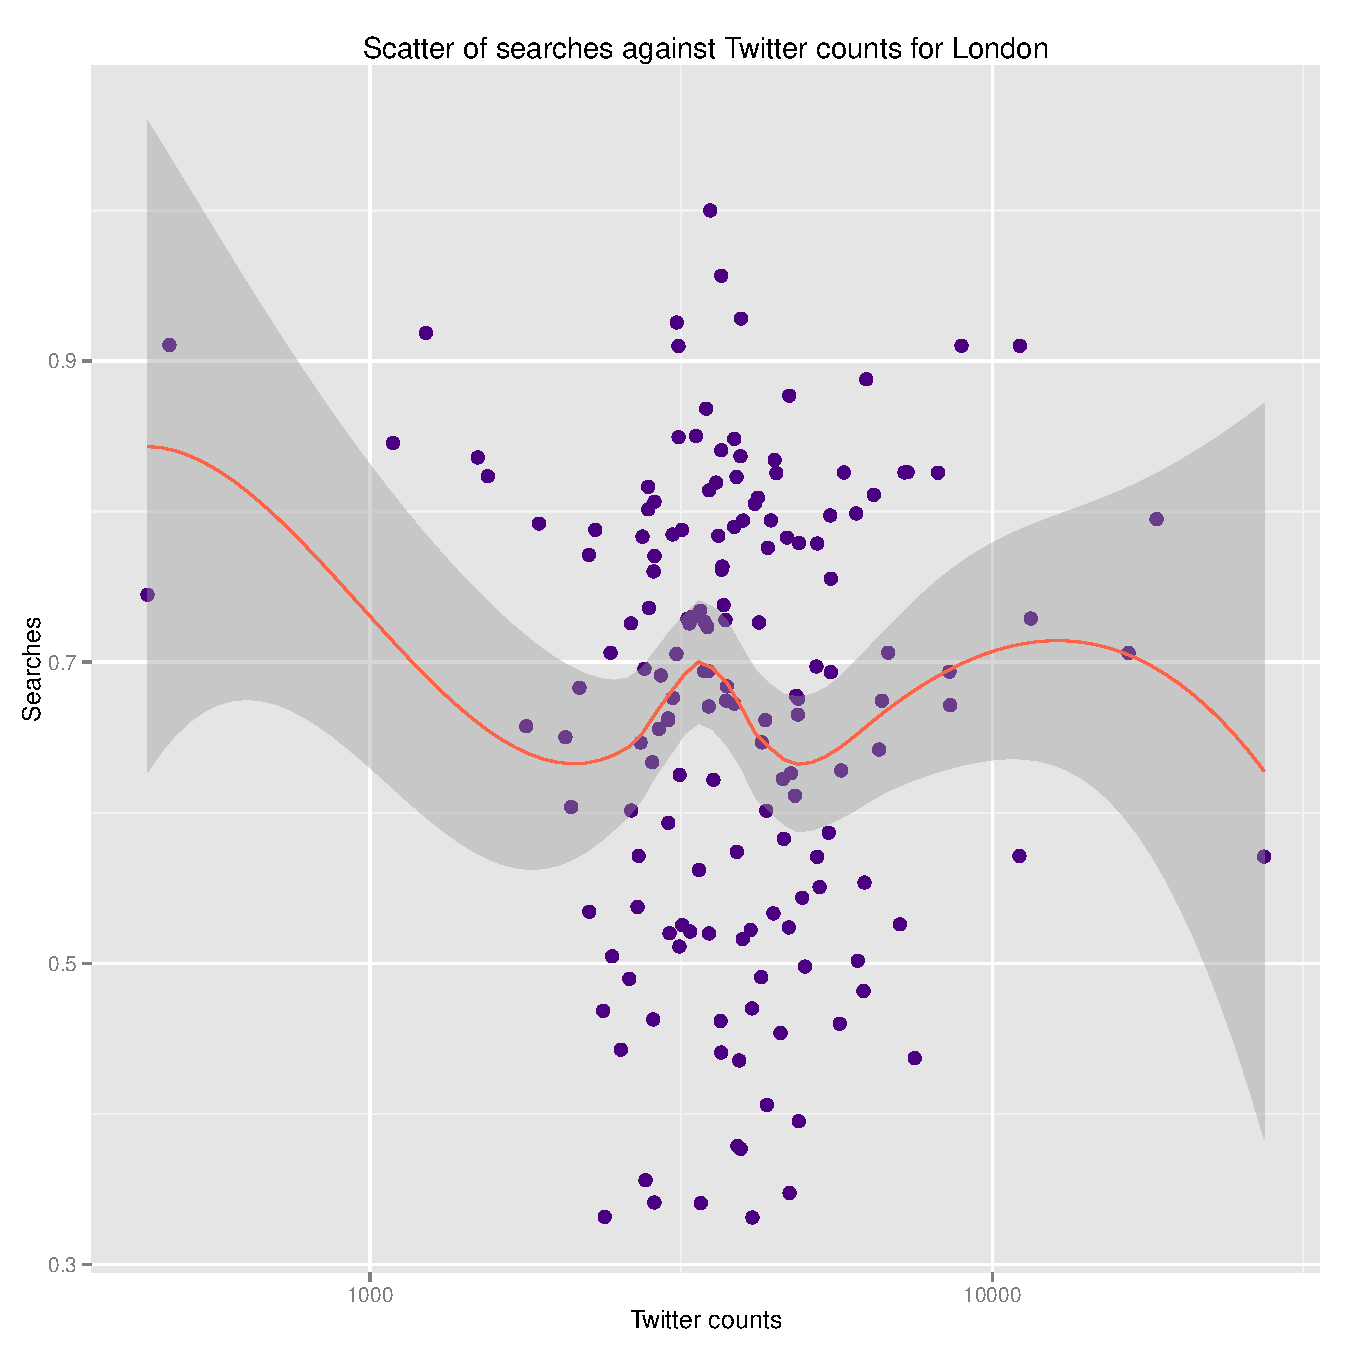
\includegraphics[width=\textwidth]{London}

There is definitely a relationship, even though not perfectly linear.

We can observe that there is a well defined cluster where the twitter counts are big and the corresponding searches are relatively big as well. We can't say with great certainty that those two are perfectly correlated, because correlation does not imply causation. So what we needed to do was to delve even further and build a model that would work with those.

%So we can certainly say that those variables are correlated, but the outliers push the coefficient down quite a significant amount. The interesting part of this scatter plot for us is the top right corner. We are interested in those abnormal Twitter counts, which correspond to high number of redirects. Another interesting thing to explore would be to see if we correlate the mentions on the social network with the redirects from the next day. That will assume a certain lag factor, which is reasonable as sometimes an event should not effect the redirect counts till the next day when it's picked by all the major media. 

Paris was one of the most popular destinations so it was quite interesting to see what the relation is there. The Pearson test yields the following values for Paris:
\begin{quotation}
In [24]: r\_value, p\_value

Out[24]: (-0.25, 0.0047)
\end{quotation}
\newpage
And here is the scatter plot:

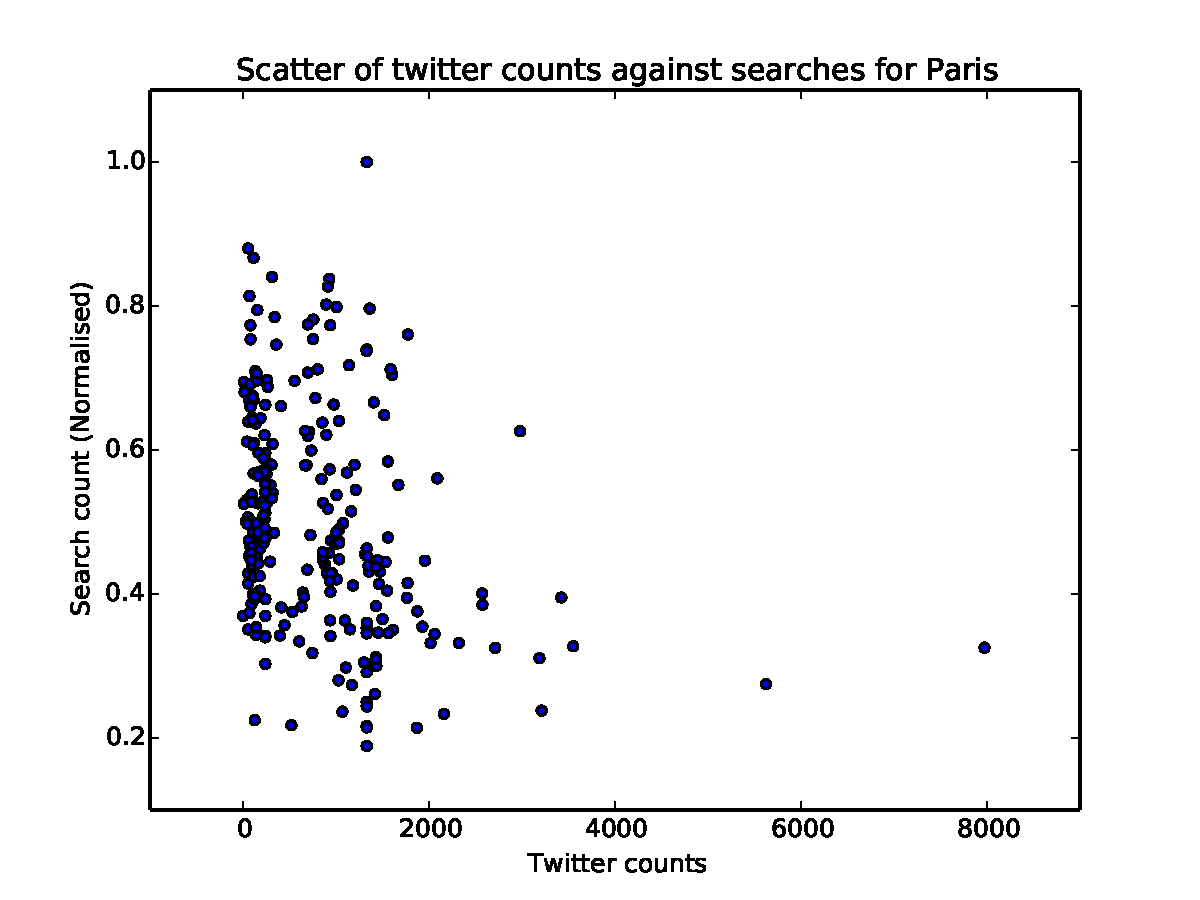
\includegraphics[width=\textwidth]{Paris}

Here we do see that indeed the correlation is relatively small and negative. 

As we can see each of the different cities shows a different behaviour. The implications of that are that the approach we take to building the model must be more versatile - we will aim to build one model for the overall numbers and models on a per city basis.

\section{Cleansing the data}

As mentioned, every time you depend a few external data source there will be some problems with the data, caused by several things. 

In this project there were a couple of major sources of problems:
\begin{enumerate}
\item The script that collects data from the Streaming API.
\item The searches data coming from Skyscanner being incorrect or partial - not spanning the full date range.
\end{enumerate}

The dates with incomplete data or missing data altogether can seriously impact any regression or statistical test, so it was vital to tidy up the data set by backfilling it. I applied the Last 4 Fridays forecasting algorithm mentioned in the following chapter in order to make the dataset more consistent and easier to work with. 

The interesting part was that it completely change the results from the test. For London the values returned by the Pearson test are now:

\begin{quotation}
In [23]: r\_row, p\_value

Out[23]: (-0.23, 0.02)
\end{quotation}

That is quite interesting and it has a lot of implications on the models we will use afterwards to correlate the two variables. 
We might have to add a certain "lag" factor to this, which will offset the tweets by correlating the numbers extrapolated from Twitter with the numbers and match them against searches from the following day.

%\section{Top features} 

%The idea here is to extract the top N features from the tweet and use them in the logistic regression model that we will build to predict the search counts. I plan on working on this in the next couple of weeks.


\chapter{Models}
\label{chap:model}

\section{The baseline model}

The baseline model for predicting the number of redirects Skyscanner has on a daily basis is called Last 4 Fridays. 
It works in the following way:
\begin{enumerate}
\item We want to predict the number of redirects/searches for this Friday.
\item We take the number of redirects/searches Friday from last week, the week before, etc, until we have the counts form the previous 4 weeks for the corresponding day.
\item We then assign weights to those 4 numbers and assign weights - the most recent one will get the highest weight, the one after about a half and so on. The exponential weighting scheme captures short term seasonality.
\end{enumerate}

This model was tested out against more complex classifiers like ARIMA and Autoregressive Vector Methods and it performed really well, but unlike the others it was many times simpler to program and maintain.

\section{Last 4 Fridays + Twitter Counts}

The first model I build was not a radical new approach, but rather an increment on the previous one.

I generated a list of tuples which contained the following information:
\begin{itemize}
\item Twitter count for the place - how many times it was mentioned in conjunction with a travel term.
\item Same day of the week from last week
\item Same day of the week from 2 weeks ago
\item Same day of the week from 3 weeks ago
\item Same day of the week from 4 weeks ago
\end{itemize}

What this is is a version of Last 4 Fridays which now has Twitter Counts. Instead of using the exponential weights from the previous algorithm I let LASSO determine their weights.
With LASSO I had weights for each of the 272 cities. After measuring the RMSEs for the L4F algorithm and expanded version with Twitter Counts the former performs better on 193 of the 272 cities. In the top 10 L4F+Twitter performs better on 2 out of 10. 

Dublin which is in the 4th spot in terms of volumes is quite interesting. I plotted out the counts against searches just to see how it looks:

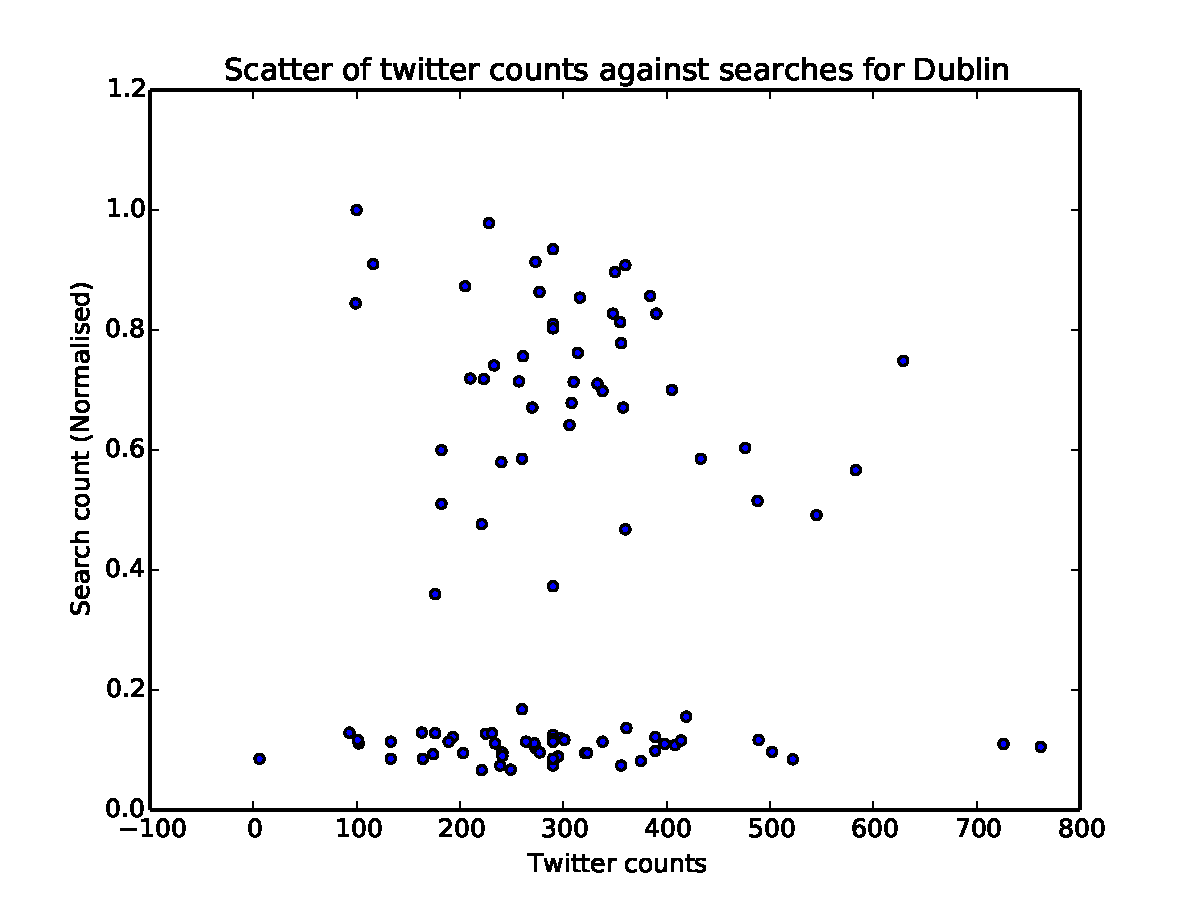
\includegraphics[width=\textwidth]{Dublin}  

\newpage
\section{Results}

And here are the results for the top 10 destinations by volume (they have the highest RMSEs).

\begin{tabular}{ l | r | r }
City	& RMSE L4F+Twitter &RMSE L4F \\
\hline
London & 3335.869525 & 3160.05886 \\
Paris	 & 939.1057276 & 921.6785638  \\
Barcelona & 920.6831066 & 897.6473097  \\
Milan & 760.3436591 & 760.9286718  \\
Rome & 710.7052517 & 705.8388511  \\
Manchester & 574.8431422 & 572.4116201  \\
Dublin & 514.584231	 & 527.884409  \\
Amsterdam & 550.2254781 & 516.2054596  \\
Tenerife & 544.6187529 & 502.0270723  \\
Moscow & 499.1803266 & 495.2139406  \\
\end{tabular}


This is quite a good start considering the fact that all the weights were automatically determined by the LASSO algorithm and the fact that I have only about 130 data points so far (130 days).

\section{Future improvements}

The next on the list is to expand the feature set with more features from Twitter such as:


\begin{itemize}
\item Specific words.
\item Trending event or not.
\item Investigate whether sentiment will be useful here.
\end{itemize}

With those I'll be able to better the model and reduce the RMSE across the whole board and hopefully beat the current prediction algorithm for more than 80\% of the examples.


\chapter{Future work}
\label{chap:future-work}


%\chapter{Timeline}

%The timeline for the next 3 months is the following:
%\begin{enumerate}
%\item Better the existing model and continue with the tests. .
%\item Add more features to the set of inputs.
%\item Work on both approaches:
%\begin{itemize}
%\item Explain spikes in searches by looking at historical tweet data
%\item Or try to predict the spikes in the first place
%\end{itemize}
%\item Final draft done by mid-March.
%\item Submit dissertation the final week of March.
%\end{enumerate}

\begin{thebibliography}{10}

\bibitem{TwitterNewsWire}
	Twitter, \emph{Twitter as a news-wire}, \\
	{\url{https://blog.twitter.com/2008/twitter-news-wire}}

\bibitem{TwitterResearch}
	Twitter Research,
	\emph{A collection of publications using Twitter data}, \\
 	{\url{https://sites.google.com/site/twitterresearch09/twitter-papers}}

\bibitem{Miles}
	Miles Osborne, \emph{Social media papers}, \\
	{\url{http://homepages.inf.ed.ac.uk/miles/sm-papers.html}}
	
\bibitem{Petrovic2012}
  	\emph{Real-time Event Detection in Massive Streams, Sasa Petrovic}, 2012, School of Informatics, University of Edinburgh \\
	{\url{http://homepages.inf.ed.ac.uk/s0894589/petrovic-thesis.pdf}}
  
  
\bibitem{Hamletkdd03}
 	Etzionni, Tuchinda, Knoblock and Yates, \emph{To Buy or Not to Buy: Mining Airfare Data to Minimize Ticket Purchase Price}, 2003, \\
  	{\url{http://knight.cis.temple.edu/~yates/papers/hamlet-kdd03.pdf}}
	
\bibitem{ijcai}
	William Groves and Maria Gini, \emph{Optimal Airline Ticket Purchasing Using Automated User-Guided Feature Selection}
	{\url{http://ijcai.org/papers13/Papers/IJCAI13-032.pdf}}

\bibitem{code}
	Stefan Sabev, Code for Inf Project,\\
	{\url{https://github.com/SSabev/HonsProject/}}

\end{thebibliography}

\end{document}
